
\documentclass[a4paper,10pt]{article}
\usepackage{graphicx}
\usepackage{fullpage}
\usepackage{fancyhdr}
\usepackage{fourier}
\usepackage{framed}
\usepackage{booktabs}
\usepackage[hyphens]{url}
\usepackage{hyperref}
\usepackage{array}
\usepackage[justification=justified,singlelinecheck=false]{caption}
\usepackage{float}
\usepackage{todonotes}
\usepackage{subcaption}

\setlength{\headsep}{20pt}
\setlength{\headheight}{12pt}
\pagestyle{fancy}
\setlength{\parskip}{10pt plus 1pt minus 1pt}
\sloppy
%TODO: remove following....
\overfullrule=1mm

%\title{BugBuilder Users Guide}

%\author{James Abbott (j.abbott@dundee.ac.uk)}
%\date{}
\begin{document}
\begin{titlepage}
\begin{center}
  \bfseries
  \huge BugBuilder User Guide
  \vskip 0.1in
  \textsc{\normalsize Version 1.00 }
  \vskip 0.1in
  \textsc{\normalsize James Abbott (j.abbott@dundee.ac.uk)}
\end{center}

%\renewcommand{\baselinestretch}{0.25}\normalsize
%\maketitle
\tableofcontents
\renewcommand{\baselinestretch}{1.0}\normalsize
\end{titlepage}
\newpage
\graphicspath{ {images/} }

\section{Introduction}

BugBuilder is a pipeline enabling assembly and annotation of microbial genomes
from high-throughput sequence data. It is designed to minimise manual work in
creating annotated, draft genome assemblies ready for submission to public
databases.  BugBuilder offers a configurable framework capable of supporting a
number of different assemblers and scaffolders which are selectable at runtime.
These provide support for all assemblyh of data generated with all common
sequencing platforms (Illumina, 454, IonTorrent, PacBio and MinIon), including
hybrid assembly between e.g. Illumina and PacBio sequences.  It is implemented
in Perl and has been tested on Red Hat derived Linux distributions, however
should work on any Unix-like operating system which supports the prerequisite
software components.


BugBuilder is available from the BugBuilder home page at\\*
\url{http://www.imperial.ac.uk/bioinfsupport/software/BugBuilder}. The code is
maintained in a GitHub repository which can be found at
\\*\url{https://github.com/jamesabbott/BugBuilder}.  

\section{Quick Start Guide}

\subsection{Installation}

Installation and configuration of a standalone instance of BugBuilder requires
a degree of knowledge of Linux software installation and management, and
installation of a considerable number of prerequisite packages, so it is
recommended to initially try out BugBuilder using the pre-configured virtual
machine image (see section \ref{sec:vminstall}: Virtual Machine Installation),
which requires a minimal amount of setup work. 

\subsection{Running BugBuilder}

Once BugBuilder is available on your system, you can perform an assembly of a
paired-end sequencing run simply by entering the command:

\begin{verbatim}
BugBuilder --fastq1 read1.fastq --fastq2 read2.fastq --platform illumina
\end{verbatim}

where 'read1.fastq' contains the reads from the first read of the pair, and
read2.fastq contains the second read, and the 'platform' argument defines the
sequencing platform used to generate the reads. If your sequence was generated
from a fragment library rather than a paired-end library, the '--fastq2'
argument should be omitted.  BugBuilder will proceed to carry out the assembly,
reporting it's progress to the screen. Once complete, the generated outputs
will be written to a new directory within the current working directory. 

If you have an appropriate reference genome sequence (ideally a complete genome
from the same genus, or preferably species), this can be used to guide the
scaffolding process typically producing fewer scaffolds. The reference genome
needs to be provided in fasta format, and can be included in the analysis using
the {\tt '--reference'} argument:

\begin{verbatim}
BugBuilder --fastq1 read1.fastq --fastq2 read2.fastq \
    --reference myreference.fasta --platform illumina
\end{verbatim}


Your BugBuilder installation may have been configured with multiple assemblers
and scaffolders.  Certain assemblers are appropriate, or perform better, with
particular sequence types, and BugBuilder can select the most appropriate
tools for your assembly based on the sequencing platform used, and the length
of your sequence reads.  These appropriate tools for each platform are
centrally configured within the BugBuilder configuration file.  

To see which assemblers, scaffolders and platforms are configured, view
the help documentation by entering:

\begin{verbatim}
[jamesa@codon ~]$ BugBuilder --help

Welcome to BugBuilder

Available assemblers: SPAdes, abyss, celera
Available scaffolders: SIS, sspace, mauve
Configured platforms: 454, illumina, iontorrent, hybrid
\end{verbatim}


An appropriate assembler and scaffolder for the type of sequence available will
be selected from the configured options based on the sequencing platform
supplied using the {\tt '--platform'} argument: Alternatively, rather than
using the automatically selected tools, the assembler and scaffolder can be
directly specified using the {\tt '--assembler'} and {\tt '--scaffolder'}
arguments:

\begin{verbatim}
BugBuilder --fastq1 read1.fastq.gz --fastq2 read2.fastq.gz  --platform illumina\
    --reference myreference.fasta --assembler spades --scaffolder SIS
\end{verbatim}


\section{Installation}

There are a considerable number of prerequisite packages which are required for
BugBuilder, and a configuration file which needs to be setup to indicate the
location of the installed packages, and defines the available assemblers and
scaffolders. This can make installation a fairly complex process. A
preconfigured virtual machine is therefore available which is installed and
configured with all freely distributable packages and a script to automate the
installation of the remaining software which it is not possible to distribute
directly due to restrictive licenses. The virtual machine image should provide
a functional environment where BugBuilder can be run, however those making
heavy use of the software would benefit from carrying out a full installation
in a Linux environment.

Should a full installation be desirable, then an automated  installation script
is provided (currently only for RHEL-derived Linux installations) which will
attempt to install and configure as much of the software as possible. See
section \ref{sec:autoinstall} (Automated Installation) for details on carrying
out a scripted installation. 

Experienced Linux users may prefer to use existing installations of
prerequisite packages on their systems, or manually install the tools required.
Details on manual installation of the prerequisites and configuration of the
BugBuilder installation can be found in section \ref{sec:maninstall} (Manual
Installation).

\subsection{Virtual Machine Installation}\label{sec:vminstall}

The BugBuilder virtual machine image has been created with VirtualBox and it is
recommended that it be run in a VirtualBox environment, however the disk image
can be converted to formats appropriate for running under other virtualised
environments such as KVM or VMware.

\begin{enumerate}
\item Install VirtualBox from \url{https://www.virtualbox.org}, following the
instructions  for your operating system. 

\item Download the BugBuilder virtual machine image from
\url{http://www3.imperial.ac.uk/bioinformatics-support-service/resources/software/bugbuilder}.

\item Start VirtualBox on your machine - how to do this will vary according to
your operating system. Once running you should see a window displayed such as
that shown in figure \ref{fig:vm_install1}

\begin{figure}[!h] \fbox{\includegraphics[width=0.6\textwidth]{vm_install1}}
\caption{VirtualBox main window} \label{fig:vm_install1} \end{figure}

\item Click the 'New' icon on the toolbar to open a dialog box for creating a
new virtual machine. Enter 'BugBuilder' in the 'Name' field, then select
'Linux' from the 'Type' drop-down menu, and 'Red Hat (64-bit)' from the
'Version' menu. The window should look like that shown in figure
\ref{fig:vm_install2}. Click the 'Next' button.

\begin{figure}[H] \fbox{\includegraphics[width=0.6\textwidth]{vm_install2}}
\caption{Create virtual machine window} \label{fig:vm_install2} \end{figure}

\item The next window displayed allows the amount of memory available to the
virtual machine to be defined. Adjust the slider to set the desired amount of
memory as shown in figure \ref{fig:vm_install3}. BugBuilder has been tested with
4Gb (4096 Mb) RAM allocated to the virtual machine, which appears to be
sufficient for most situations. Allocating larger amounts of memory to the
virtual machine will result in improved performance, however it is necessary to
ensure that the selected value leaves sufficient memory for other programs
running on the computer.

\begin{figure}[H] \fbox{\includegraphics[width=0.6\textwidth]{vm_install3}}
\caption{Defining memory available to the BugBuilder virtual machine.}
\label{fig:vm_install3} \end{figure}

\item Next, the hard-disk to be used by the virtual machine needs to be
configured. Select the 'Use an existing virtual hard disk file' option, then
click the file icon alongside the dropdown menu and navigate to the
BugBuilder.vdi file you downloaded in step 2. The window should look like that
shown in figure \ref{fig:vm_install4}. Now click the 'Create' button.

\begin{figure}[H] \fbox{\includegraphics[width=0.6\textwidth]{vm_install4}}
\caption{Selecting the virtual disk image.} \label{fig:vm_install4} \end{figure}

\item \textbf{Network Configuration}: VirtualBox supports a number of different
network modes.  The network mode can be chosen by selecting the BugBuilder
virtual machine in the VirtualBox window, , clicking the 'Settings' button on
the toolbar then 'Network' in the left-hand pane of the window. The networking
mode can then be selected in the 'Attached to:' dropdown menu. (see figure
\ref{fig:vm_network_settings}).

\begin{figure}[H] \fbox{\includegraphics[width=0.6\textwidth]{vm_network_settings}}
\caption{VirtualBox network configuration} \label{fig:vm_network_settings} \end{figure}

The default NAT (Network Address Translation) mode will allow
the BugBuilder virtual machine to connect to other machines on the internet
i.e. to download data onto the virtual machine, however it does not allow you
to login to the virtual machine remotely (i.e. using SSH).  If you require full
network access for the virtual machine, then it will be necessary to use one of
the alternate network modes. If your network provides a DHCP server, then
'bridged networking' (which allows the virtual machine access to the network
just like a physical machine) is probably the best configuration to use,
although this depends upon your network configuration. Please contact your
local network administrator to determine the most appropriate way to configure
networking on your virtual machine.

\end{enumerate}

\subsubsection{Starting the Virtual Machine}

The virtual machine can be started by selecting the BugBuilder virtual machine
in the VirtualBox interface, and clicking the 'Start' icon on the toolbar.  The
virtual machine will then be booted in a new indow, and when complete will
appear as shown in figure \ref{fig:vm_running}.

The login screen displays a file-system usage indicator, which shows the amount
of space consumed on the vitual machine's disk. By default the disk is
configured to expand up to 50Gb in size.

Below this is shown the IP address allocated to the virtual machine. If your
networking is configured in a mode which supports connecting directly to the
virtual machine via the network (i.e. bridged networking), you can use this IP
address to establish your connections.

\begin{figure}[H] \fbox{\includegraphics[width=0.6\textwidth]{vm_running}}
\caption{BugBuilder virtual machine following boot.} \label{fig:vm_running}
\end{figure}

\subsection{Virtual Machine Post-Installation Configuration}

The virtual machine is setup to provide a fully working BugBuilder
installation. The BugBuilder software is installed in {\tt /opt/BugBuilder},
with the BugBuilder scripts available on the default path. 

Certain packages can not be pre-installed in the virtual machine image due to
licensing constraints, however BugBuilder is perfectly functional without
these. The packages which can not be distributed directly are AbySS, SSpace,
GapFiller, and RNAmmer. The additional packages can be downloaded from
the sites indicated in table \ref{tab:prereq}, then copied to the
/opt/BugBuilder/src directory.  The packages can then be installed by running
the {\tt /opt/BugBuilder/bin/configure.pl} command, which will carry out the
necessary installation processes and generate an updated configuration file.

\subsection{Full Installation}

\subsubsection{Obtaining the software}

The software can be obtained from
\url{https://github.com/jamesabbott/BugBuilder} as a zip file by clicking the
'Download ZIP' button on the right of the page. Alternatively, if git is
installed on your machine you can run {\tt git clone
https://github.com/jamesabbott/BugBuilder} and the latest version of the
software will be downloaded into a 'BugBuilder' directory within your current
working directory.

\subsection{Automated Installation}\label{sec:autoinstall}

BugBuilder includes a script to automate the installation of the prerequisite
packages within the BugBuilder installation and setup the configuration file
appropriately. This has been developed and tested in a CentOS 7 environment but
should work on other RHEL-derived distributions. If you want to use existing
packages installed on your system, a manual installation and configuration
should be carried out.

The location of the extracted software is referred to in the remainder of this
document as {\tt \$BUGBUILDER\_HOME}. This can be set as an environmental
variable to allow commands in the manual to be copied verbatim by typing:

\begin{verbatim}export BUGBUILDER_HOME='path'\end{verbatim}

where 'path' is replaced by the path to the directory where the software is unpacked.

An automated installation can be carried out as follows:

\begin{enumerate}
\item Download the BugBuilder software: 
\begin{verbatim}git clone https://github.com/jamesabbott/BugBuilder\end{verbatim}
\item Change to the BugBuilder src directory:
\begin{verbatim}cd $BUGBUILDER_HOME/BugBuilder/src\end{verbatim}
\item Download the prerequisites tarball: 
\begin{verbatim}wget http://web.bioinformatics.ic.ac.uk/BugBuilder/BugBuilder_prerequisites.tar\end{verbatim}
\item Unpack the downloaded tarball
\begin{verbatim}tar xvf BugBuilder_prerequisites.tar\end{verbatim}
This will unpack the various software installation packages into the {\tt
BugBuilder/src} directory
\item Remove the tarball to save disk space (optional):
\begin{verbatim}rm BugBuilder_prerequisites.tar\end{verbatim}
\item (Optional) Download additional not-redistributable packages. RNAmmer is
an essential prerequisite for Prokka, so needs to be installed. The other
non-redistributable packages are optional, however it would be highly
recommended to add these additional packages which can significantly improve final
assembly contiguity. Additional downloaded packages should be copied into the
{\tt BugBuilder/src} directory. See table~\ref{tab:prereq} for download details
of these packages.
\item Run the automated installation script:
\begin{verbatim}$BUGBUILDER_HOME/bin/configure.pl\end{verbatim}

The script will firstly attempt to install necessary Perl modules locally
within the BugBuilder installation, following which the prerequisite software
packages will be installed. Each will be unpacked in the {\tt src}
subdirectory, then compiled and installed as necessary. Full outputs of the
installation process for each package being are recorded in the {\tt
install\_logs} directory. In the event of any issues with the installation a
package, a warning will be generated by the {\tt configure.pl} script, which
should be examined to determine the cause of the problem.

Once package installation has completed, an appropriate configuration file will
be generated. The location of a directory to use as temporary working space
will first be requested (defaulting to \/tmp). Should it not be possible for
the script to determine the location of any packages, a prompt will be
displayed requesting the path to the installation to be entered. If the package
in question is not available, just press enter to skip configuration of this
package. Following package configuration, the {\tt BugBuilder.yaml}
configuration file will be written to the {\tt etc} directory within the
BugBuilder installation, and can then be edited using a text editor if
required. Details on editing the configuration are contained in the following
section.

\end{enumerate}

\subsection{Manual Installation}\label{sec:maninstall}
\subsubsection{Operating System Packages}

Certain packages are required which can be installed from the operating systems
package repositories. Note that package names may vary between distributions.
The necessary packages are indicated in table ~\ref{tab:ospackages}, and can be
installed using the appropriate tools according to your operating system (i.e.
yum, dnf, apt).

\begin{table}[htb]
\resizebox{\textwidth}{!}{%
\begin{tabular}{lll}
\hline
\textbf {Package} & \textbf {RHEL/CentOS/Fedora Package} & \textbf {Debian/Ubuntu Package} \\
\hline
bzip2                  & bzip2                                   & bzip2 \\
gcc                    & gcc                                     & gcc \\
g++                    & gcc-c++                                 & g++ \\
fortran                & gcc-gfortran                            & gfortran \\
binutils               & binutils                                & binutils \\
patch                  & patch                                   & patch \\
libgomp                & libgomp                                 & libgomp1 \\
glibc                  & glibc.i686, glibc-headers, glibc-devel  & libc6-i386,libc6-dev \\
Perl local::lib        & perl-local-lib                          & liblocal-lib-perl\\
CPAN                   & perl-CPAN                               & perl-modules \\
Perl File::Which       & perl-File-Which                         & libfile-which-perl \\
Perl File::Find::Rule  & perl-File-Find-Rule                     & libfile-find-rule-perl \\
Perl IO::gzip          & perl-PerlIO-gzip                        & libperlio-gzip \\
Perl Text::ASCIItable  & perl-text-ASCIITable                    & libtext-asciitable-perl \\
Perl DateTime          & perl-DateTime                           & libdatetime-perl \\
Perl Statistics::Basic & perl-Statistics-Basic                   & libstatistics-basic-perl \\
Perl XML::Simple       & perl-XML-Simple                         & libxml-simple-perl \\
zilb                   & zlib, zlib-devel                        & zlib1g, zlib1g-dev \\
Expat                  & expat,expat-devel                       & libexpat1, libexpat1-dev \\
ncurses                & ncurses,ncurses-devel                   & libncurses5, libncurses5-dev \\
readline               & readline,readline-devel                 & libreadline5, libreadline5-dev \\
curl                   & curl                                    & curl \\
dos2unix               & dos2unix                                & dos2unix \\
sparsehash             & sparsehash-devel                        & libsparsehash-dev\\
openMPI                & openmpi, openmpi-devel                  & libopenmpi1.6, libopenmpi1.6-dev\\
sqlite3                & sqlite, sqlite-devel                    & sqlite, sqlite-dev\\
\hline
\end{tabular}}
\captionof{table}{Required operating system packages}
\label{tab:ospackages}
\end{table}

\subsubsection{Prerequisite Software}

A number of prerequisite software packages need to be installed prior to
running the software, which are summarised in table ~\ref{tab:prereq}. Where
version numbers are specified, these indicate the most recent version of the
software which  BugBuilder has been tested with. Previous supported versions
are indicated in the '{\tt etc/package\_info.yaml}' file. Other versions of
these packages will probably work fine, but in case of problems try using the
versions listed below. Those which are available under licenses permitting
their redistribution (indicated by the 'Bundled' column of the table) are
available in a tarball.  ('BugBuilder\_Prerequisites.tar.gz') from the
BugBuilder website.  Non-bundled packages should be downloaded from the
locations listed below.

\begin{table}[htb]
\resizebox{\textwidth}{!}{%
\begin{tabular}{llccl}
\hline
\textbf{ Package } & \textbf{ Latest Version } & \textbf { Bundled } &  \textbf { Required}  &  \textbf { Download location}\\
\hline
fastqc     & 0.11.4  & Y & Y & \href{http://www.bioinformatics.babraham.ac.uk/projects/fastqc}{http://www.bioinformatics.babraham.ac.uk/projects/fastqc} \\
sickle     & 1.210   & Y & Y & \href{https://github.com/najoshi/sickle}{https://github.com/najoshi/sickle}  \\
seqtk      & -       & Y & Y & \href{https://github.com/lh3/seqtk/archive/master.zip}{https://github.com/lh3/seqtk/archive/master.zip}\\
SPAdes     & 2.3.0   & Y & N & \href{http://bioinf.spbau.ru/spades}{http://bioinf.spbau.ru/spades}\\
ABySS      & 1.9.0   & N & N & \href{http://www.bcgsc.ca/platform/bioinfo/software/abyss}{http://www.bcgsc.ca/platform/bioinfo/software/abyss}\\
WGS Assembler & 8.3rc2 & Y & N & \href{http://sourceforge.net/projects/wgs-assembler/files/wgs-assembler/wgs-8.3/wgs-8.3rc2.tar.bz2}{http://sourceforge.net/projects/wgs-assembler} \\
AMOS       & 3.1.0   & Y & Y & \href{http://amos.sourceforge.net}{http://amos.sourceforge.net} \\
samtools   & 1.2     & Y & Y & \href{http://www.htslib.org/}{http://www.htslib.org} \\
picard     & 1.140   & Y & Y & \href{http://broadinstitute.github.io/}{http://broadinstitute.github.io} \\
SIS        & -       & Y & N & \href{http://marte.ic.unicamp.br:8747/}{http://marte.ic.unicamp.br:8747/} \\
Sspace     & 3.0     & N & N & \href{http://www.baseclear.com/landingpages/basetools-a-wide-range-of-bioinformatics-solutions/sspacev12/}{http://www.baseclear.com} \\
Mauve      & 2.4.0   & Y & N & \href{http://darlinglab.org/mauve/mauve.html}{http://darlinglab.org/mauve/mauve.html} \\
GapFiller  & 1.10    & N & N & \href{http://www.baseclear.com/landingpages/basetools-a-wide-range-of-bioinformatics-solutions/gapfiller/}{http://www.baseclear.com} \\
R          & 3.2.2   & Y & Y & \href{http://www.r-project.org}{http://www.r-project.org} \\
Prokka     & 1.5.2   & Y & Y & \href{http://www.vicbioinformatics.com/software.prokka.shtml}{http://www.vicbioinformatics.com/software.prokka.shtml} \\
Aragorn    & 1.2.36  & Y & Y & \href{http://mbio-serv2.mbioekol.lu.se/ARAGORN/}{http://mbio-serv2.mbioekol.lu.se/ARAGORN} \\
Prodigal   & 2.60    & Y & Y & \href{http://prodigal.ornl.gov}{http://prodigal.ornl.gov} \\
HMMER3     & 3.1b1   & Y & Y & \href{http://hmmer.janelia.org}{http://hmmer.janelia.org} \\
RNAmmer    & 1.2     & N & Y & \href{http://www.cbs.dtu.dk/cgi-bin/sw_request?rnammer}{http://www.cbs.dtu.dk} \\
Infernal   & 1.1rc2  & Y & Y & \href{http://infernal.janelia.org}{http://infernal.janelia.org} \\
barrnap    & 0.6.0   & Y & Y & \href{http://www.vicbioinformatics.com/software.barrnap.shtml}{http://www.vicbioinformatics.com/software.barrnap.shtml} \\
Blast+     & 2.2.31+ & Y & Y & \href{http://blast.ncbi.nlm.nih.gov/Blast.cgi?CMD=Web\&PAGE_TYPE=BlastDocs\&DOC_TYPE=Download}{http://blast.ncbi.nlm.nih.gov/Blast.cgi} \\
BWA        & 0.75a   & Y & Y & \href{http://bio-bwa.sourceforge.net}{http://bio-bwa.sourceforge.net} \\
MUMmer     & 3.22    & Y & Y & \href{http://mummer.sourceforge.net/}{http://mummer.sourceforge.net} \\
tbl2asn    & -       & Y & Y & \href{ftp://ftp.ncbi.nih.gov/toolbox/ncbi\_tools/converters/by\_program/tbl2asn/}{ftp://ftp.ncbi.nih.gov} \\
circleator & 1.0.0rc4 & Y & Y & \href{http://jonathancrabtree.github.io/Circleator/}{http://jonathancrabtree.github.io/Circleator/} \\
\hline
\end{tabular}}
\captionof{table}{Required software packages}
\label{tab:prereq}
\end{table}

\subsubsection{sam2afg}

The {\tt sam2afg} script produced by Shaun Jackman (Canada's Michael Smith
Genome Science Centre) is used in the conversion of assemblies to AMOS's bank
format. This script is available either as part of the ABySS distribution
(where it is named {\tt 'abyss-sam2afg'}), or in the AMOS git repository (named
{\tt 'sam2afg'}, but is not yet available in a released AMOS version. The AMOS
tarball available in the prerequisites bundle is therefore based on the git
repository which includes this script. 

It is necessary to modify this script with the patch located in the '{\tt src}'
directory of the BugBuilder distribution in order for it to be able to use
alignments generated using 'bwa mem' (which BugBuilder carries out when using
reads \textgreater 100 bp) as follows:

\begin{verbatim}
[jamesa@codon ~]$ cd /path/to/samtoafg 
[jamesa@codon ~]$ patch abyss-samtoafg src/sam2afg.patch
\end{verbatim}

This patch has been submitted to the AMOS developers, and hopefully will be made
available directly in future AMOS/ABySS releases which will make this stage
unnecessary in future.

\subsubsection{Perl Modules}

BugBuilder also makes use of some non-core Perl modules which need to be
installed. These can be installed either using appropriate operating system
packages,where available, or directly from CPAN using CPAN/CPANPLUS modules.The
required modules are:

\begin{itemize}
  \setlength\itemsep{0em}
  \item BioPerl 
  \item Bio::FeatureIO
  \item File::Copy::Recursive
  \item File::Tee
  \item Parallel::ForkManager
  \item YAML::XS
  \item Statistics::Basic
  \item Test::More
  \item Archive::Extract
  \item Archive::Tar
  \item Archive::Zip
  \item Digest::MD5
  \item Time::Piece
  \item Clone
\end{itemize}

The configure.pl installation script will attempt to install these itself
during automated installations. These can be installed manually from individual
modules downloaded from CPAN, or if the CPANPLUS module is available, the
following command  should install all the required modules:

\begin{verbatim}
 cpanp install Archive::Extract Archive::Tar Archive::Zip BioPerl
   Digest::MD5 File::Copy::Recursive File::Tee Statistics::Basic
   Test::More Parallel::ForkManager
\end{verbatim}

\subsection{Downloading Example Data Sets}
\label{sec:samples}

A number of example data sets can be downloaded from public repositories to
demonstrate the use and capabilities of BugBuilder with readily available data.
Run the {\tt 'bin/download\_sample\_data'} script. When run without arguments,
this will display a list of sample data sets which are available to download
from the ENA. All available datasets can be download by passing the {\tt --all}
argument to the script, otherwise individual datasets can be obtained by
passing the {\tt --dataset [name]} argument. By default, example datasets will
be downloaded into the {\tt examples} directory within the BugBuilder
installation, alternately the destination directory can be specified using the
{\tt --dir} argument. 


\section{Pipeline Workflow}
\label{sec:Workflow}

The BugBuilder workflow carries out all the tasks necessary to create an
annotated genome assembly from fastq format sequence data. The only other data
required is the identity of the sequencing platform used to generate the data,
and optionally a reference genome sequence.

\subsection{Pipeline Inputs}

BugBuilder supports either using reads from fragment libraries i.e. single
unpaired reads, or mate-pair libraries. Paired reads should be provided as a
pair of non-interleaved fastq files (i.e. in two separate fastq files, rather
than one fastq file with alternating read1/read2 sequences). Reads generated
with a long-read sequence platform (i.e. PacBio, MinION) can also be provided
separately, allowing with stand-alone assembly, or a hybrid assembly with i.e.
Illumina reads.  Additionally, a fasta format reference sequence from a closely
related organism can be provided to assist with scaffolding or orientating the
generated contigs, to improve the larger scale structure of the assembly.

\subsection{Pipeline Outputs}

The pipeline produces annotated contig/scaffold sequences in EMBL format and an
AGP 2.0 format file describing the scaffold structure which are appropriate
for submission to the ENA. If a reference genome has been provided, comparisons
of the assembly against this reference will also be generated using MUMmerplot
and BLAST in a format appropriate for viewing using the Artemis Comparison Tool
(\url{www.sanger.ac.uk/resources/software/act/}). A graphical map of the
completed assembly will also be produced using Circleator. 

\subsection{Workflow}

\begin{figure}[ht] \fbox{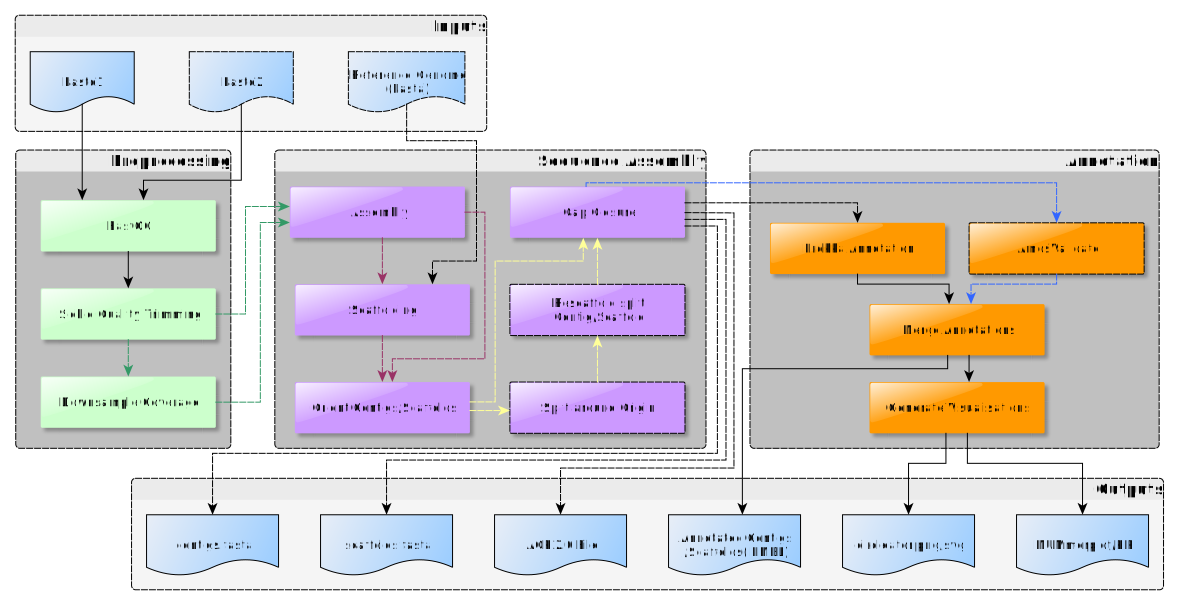
\includegraphics[width=0.9\textwidth]{BugBuilder_Workflow}}
\caption{BugBuilder Workflow} \label{fig:BugBuilderWorkflow} \end{figure}

The overall BugBuilder workflow is shown in Figure
~\ref{fig:BugBuilderWorkflow}. The core workflow is indicated by solid lines,
with hashed lines indicating optional or conditionally run parts of the
pipeline (i.e. depending upon availability of a reference genome sequence). 

\subsection{Sequence QC}

Sequence quality is key to obtaining good \textit{de-novo} assemblies. A
quality assessment of the provided sequence reads will be carried out using
FastQC, and the summary results generated displayed on the console. The full
FastQC report will be available at the end of the BugBuilder run, and should be
examined to determine the cause of any reported QC failures. 

Early high-throughput sequence assemblers ignored sequence quality scores,
however quality scores are now taken into account by some assemblers. Providing
an assembler which does not utilise the quality scores with low quality
sequence can have a significantly detrimental effect on the results of the
assembly. To ensure that any assemblers which do not use these scores are only
given good quality sequence, the sequence reads are first trimmed to a
phred-score of Q20, discarded lower quality sequence. Due to the differing
error profile inherent in long-read sequence technologies (i.e. PacBio,
MinION), sequence trimming is not currently applied to data from these
platforms.

\subsection{Downsampling}

Somewhat counter-intuitively, increasing sequence coverage will not necessarily
lead to an improvement in assembly quality. De-brijn graph based assemblers
such as ABySS and SPAdes will typically show improvements in assembly up to
around 50x coverage with prokaryotic organisms, with progressively smaller
improvements as coverage is increased. Rather than continuing to show
improvement at high coverage, assemblies will instead tend to show an increase
in incorrect bases, which is a result of a errors starting to accumulate at the
same loci. This problem can be avoided by downsampling the input sequences to a
defined coverage level. In order to determine coverage, BugBuilder needs an
estimation of the size of the target genome, which can be determined either
from a provided reference genome sequence, or by being passed the
{\tt '--genome\_size'} command line argument. If genome coverage is determined to be
above a threshold defined by the {\tt '--coverage'} command line argument
(default value: 100), then the reads are downsampled to the required coverage
level.

\subsection{Assembly}

The job of glueing together the huge number of sequence reads generated during
a sequencing experiment is handled by a tool known as an assembler. There are
now a considerable number of assemblers available capable of producing good
assemblies from high-throughput sequencing of microbial genomes. The assembly
problem is not entirely solved, however, and new and improved assemblers are
regularly being released. Rather than base BugBuilder around a specific
assembler, it has instead been developed as a framework which various different
assemblers can be plugged into, allowing the assembly component to be readily
updated as new algorithms are made available.  

There are three main classes of assembler in common usage today, the de Bruijn
graph based assembler (i.e. SPAdes, ABbyss, Velvet), consensus overlap-graph
based assemblers (i.e. Mira, Celera assembler) and string-overlap graph
assemblers (i.e. SGA). The different types of assembler tend to work better
with different sequence type i.e. de Bruijn assemblers typically produce the
best results from short-read data, whereas longer reads will often benefit from
an overlap-graph based approach.  BugBuilder is made available with
configurations for the SPAdes, ABySS and wgs-assembler (CABOG/PBcR) assemblers,
however alternative assemblers may have been configured in your installation.

\subsubsection{Assembly with Multiple Assemblers}
\label{subsec:multiassem}

Assemblers typically break contig sequences where sequences become repetitive
and difficult to extend unambiguously. Different algorithms will break contigs
in different locations, hence it is sometimes possible to get better coverage
of a genome by combining multiple assemblies. BugBuilder supports running two
independent assemblers, and merging the results (using minimus from the AMOS
package). While this approach can produce better genome coverage, it does
introduce an addition means of introducing misassemblies, and can result in
less contiguous assembles, albeit covering a greater proportion of a genome. 

Note that this functionality was included in BugBuilder
prior to the SPAdes assembler being commonly used. SPAdes carries out multiple
assemblies using different k-mers which effectively carries out a similar job
to BugBuilder's use of multiple assemblers, and typically achieves similar (or
better) quality results. This functionality has been retained in BugBuilder
since there may be use cases where it is effective, however it would generally
be recommended to use SPAdes for assembly in preference to running multiple
assemblers.


\subsection{Scaffolding}

The primary job of an assembler is to build a series of contiguous sequences
from the separate sequence reads, extending these sequences as far as possible
until it becomes no longer possible to unambiguously extend the contig
sequences. Based upon the location of paired reads on different contigs, even
when it is no longer possible to extend a contig sequence any further, it can
sometimes be possible to make an association between  contigs and get an idea
of the size of the gap between them. This is a process known as scaffolding,
which is undertaken by some assembly algorithms, but which may also be carried
out separately by standalone scaffolding algorithms.

If scaffolds are produced by the selected assembler, these will be available
for downstream processes, however if a standalone scaffolder is selected, the
outputs of this will be used in preference to those from the assembler. 

Scaffolding is the process through which sequence contigs can be arranged to
give an impression of the larger-scale organisation of a genome. Typically this
is carried out using evidence of association between contigs obtained from
read-pairs located on different contigs (see figure
~\ref{fig:ReadPairScaffolding}). This approach tends to have limited success
with bacterial genomes sequenced with a single short-insert library since the
library insert size is insufficient to span repetitive regions within the
genome. An alternative approach which has had considerable success with
microbial genomes is to align the generated contigs against the genome sequence
of a closely related organism, and use this evidence to order and orientate the
contigs.

\begin{figure}[ht]
\fbox{\includegraphics[width=0.9\textwidth]{paired_read_scaffolding}}
\caption{Scaffolding contigs with read-pair information}
\label{fig:ReadPairScaffolding}
\end{figure}

As with assembly algorithms, BugBuilder allows scaffolding algorithms to be
preconfigured and selected at runtime rather than tying the pipeline into one
algorithm. BugBuilder is preconfigured to work with the SSPACE, SIS and Mauve
scaffolders. SSPACE utilises read-pair information to generate scaffolds, and
with microbial genomes typically does not outperform the scaffolding algorithms
build into assembly tools. SIS is a tool which utilises MUMmer to align the
contigs against a reference genome, and utilises this information to determine
the order and organisation of contig sequences. Mauve takes a similar approach
only using it's own alignment algorithm. 

The scaffolder configuration allows for a set of default arguments to be passed
to the scaffolder command line, defined using the '{\tt default\-args}'
attribute. This can be overridden at runtime by passing arguments with the
command-line argument '{\tt --scaffolder\-args}'. 

The advantage of read-pair based scaffolding algorithms is that they are not
biased by external factors, whereas alignment against a reference genome may
result in an assembly which is artificially skewed towards the organisation of
the reference organism. Reference guided scaffolding typically produces far
lower number of scaffolds, however.

\subsection{Scaffold Orientation and Origin Identification}

Some scaffolders will output scaffolds in the correct orientation, but this
behaviour varies between scaffolders, and those which just make use of
read-pair information have no way of determining the correct orientation of the
various scaffolds. If a reference genome is provided, BugBuilder will then
align the scaffolds against this reference to ensure they are correctly
orientated. 

Contigs produced during assembly will typically span the origin of replication.
BugBuilder will attempt to locate the origin within the assembled scaffolds
based upon the reference genome alignment, and will split the scaffolds at this
point, relocating the upstream region to the other end of the assembly.

\subsection{Gap Closure}

Once scaffolds have been ordered, it can be possible to further close some gaps
between contigs where the assembler was not able to unambiguously extend the
contig. BugBuilder uses the GapFiller tool produced by BaseClear for this stage
of the workflow. GapFiller iteratively aligns reads from the fastq files
against the scaffolds, looking for read-alignments which hang off the end of
the contiguous sequences. After a number of cycles, some of these extensions
may end up spanning the gap between contigs.

Gap closure can be controlled using the {\tt --gap-fill} command line option.
By default, if GapFiller is installed in your BugBuilder installation then gap
filling will be carried out on any assembly with less than 150 contigs if a
reference genome sequence is provided. For performance reasons, GapFiller will
only be run on assemblies containing more than 150 contigs if the {\tt
--gap-fill} command line argument is provided. To prevent GapFiller from
running, add the {\tt --no-gap-fill} argument to the command line.

\subsection{AGP Generation}

Scaffold structures for genomes submitted to public databases need to be
defined in AGP ('A Golden Path') files. This is a text file which species the
order and orientation of the contigs on the scaffolds, the sizes of the gaps
between contigs and the kind of evidence used to establish the ordering.
BugBuilder processes the scaffolds to extract fresh contig sequences by
splitting the scaffolds around 'N's. The public database require a minimum
contig size of 200 bp, and do not allow runs of more than 10 'N's in contig
sequences. Contigs shorter than 200 bp are therefore discarded, and if these
are within scaffolds the scaffold gaps are extended to take account of the
removed sequence.  The type of evidence for the gaps is added according to the
value of the 'linkage-evidence' attribute in the  scaffolder configuration.

\subsection{Annotation}

The assembled sequences are annotated using the Prokka package, which utilises
a number of tools for \textit{de-novo} CDS, tRNA and rRNA  identification. It
uses organism specific databases to aid the annotation and can be passed
arguments to indicate the genus and species of the genome being annotated.
BugBuilder similarly allows these arguments to be specified on the
command-line, using the {\tt --genus} and {\tt --species} arguments, and passes
these values to Prokka if they are provided. If scaffolds have been generated
during the assembly process, then the annotation will be applied to them,
otherwise the contig sequences will be used.

\begin{verbatim}
  BugBuilder --fastq1 read1.fastq --fastq2 read2.fastq  \
    --reference myreference.fasta --genus Streptococcus --species pyogenes
\end{verbatim}

Prokka post-processes the annotations to identify terms which do not conform to
the NCBI recommendations, and corrects these. 

\subsection{Outputs}

The resulting output files are copied into a directory within the directory
from which BugBuilder was launched. If genus/species/strain names have been
provided, the directory will be named \\ {\tt
BugBuilder\_genus\_species\_strain}. If the full contents of the working
directory are required, for example for debugging purposes, specifying the {\tt
--keepall} command-line argument will copy the full contents of the directory
rather than just the final output files.

\subsection{Output Visualisation}

BugBuilder will additionally generate a number of graphical visualisations of
the resulting assembly to assist in interpretation of the outputs.

\subsubsection{MUMmerplot}

If a reference genome sequence has been  provided, an alignment of the
assembled scaffolds against the reference sequence will be carried out using
MUMmer's nucmer algorithm, which is then used to generate a graphical plot of
similarity between the sequences (somewhat akin to a dotplot - see figure
~\ref{fig:mummerplot}). This will be found as a png format image file located
in the output directory named {\tt refname\_vs\_queryname.png}. The reference
genome is represented along the X-axis of the plot, and the assembly on the
Y-axis, while regions of similarity between the sequences are drawn in red for
sequences aligned in the same orientation, or blue for reversed alignments.
This provides a useful overview of the large-scale organisation of an assembly
in comparison to the reference sequence, and can help identify regions of
misassembly. Additionally, a second plot will be generated displaying the
percentage identity of the alignment along the length of the reference sequence
(figure ~\ref{fig:mummerplotpip}). This can help identify the degree of
conservation present between the genomes.

\begin{figure}[htbp]
  \begin{subfigure}[b]{0.45\textwidth}
    \includegraphics[width=\textwidth]{MUMmerplot}
    \caption{Similarity Plot}
    \label{fig:mummerplot}
  \end{subfigure}
  \hfill
  \begin{subfigure}[b]{0.45\textwidth}
    \includegraphics[width=\textwidth]{MUMmerplot_pip}
    \caption{Percentage Identity Plot}
    \label{fig:mummerplotpip}
  \end{subfigure}
  \caption{MUMmerplot outputs}
\end{figure}

\subsubsection{ACT Comparison}

A comparison is also carried out between the reference genome and the
scaffolded assembly using NCBI BLAST, output in a tab-delimited format
appropriate for loading into the Artemis Comparison Tool (ACT). The allows a
fine-grained comparison of the genomes to be carried out, with regions of
similarity and reorgansations clearly indicated in the context of the sequence
annotations. ACT can be obtained from 
\href{http://www.sanger.ac.uk/resource/software/act}{http://www.sanger.ac.uk/resources/software/act}. 

\subsubsection{Circleator Visualisaion}

A graphical visualisation of the assembly and gene locations is produced using
Circleator (~\ref{fig:circleator}). The output is generated as both SVG and PNG format, named {\tt
circleator.svg} and {\tt circleator.png}. This is a circular representation of
the assembly, with the scaffolds laid out sequentially around the circle
(indicated by dark-blue bands). Surrounding this is a GC plot, while within
the scaffold-ring are two rings indicating the location of genes on the
positive and negative strands respectively. tRNA locations are highlighted by
labels within the circle. The circleator output can be customised by editing
the cirleator template ({\tt \$BUGBUILDER\_HOME\slash etc\slash circleator.cfg.tmp}) in accordance
with the Circleator documentation
(\href{http://jonathancrabtree.github.io/Circleator/documentation.html}{http://jonathancrabtree.github.io/Circleator/documentation.html}).
Note that if the Circleator configuration is edited it should be tested by
running Circleator outside of BugBuilder to ensure the template is valid and
produces the desired results.

\begin{figure}[ht] 
  \centering
  \fbox{\includegraphics[width=0.7\textwidth]{circleator}}
  \caption{Circleator Genome Visualisation} 
  \label{fig:circleator} 
\end{figure}

\section{Submission vs Draft Modes}

BugBuilder can be run in modes targeted at producing output suitable for submission to public
databases, or for carrying out further finishing work. The mode to run in is defined using the {\tt
--mode} command line argument, which accepts values of either 'submission' or 'draft'. The
default mode is 'submission'.

\subsection{Submission Mode}

Submission mode creates output suitable for submission to the ENA, with contigs \textless200 bp removed,
and no consecutive runs of more than 10 'N's in contig sequences. This is the default mode. 

\subsection{Draft Mode}

Draft mode does not remove short contig sequences from the assembly, retaining
the full output of the assembler. In order to highlight potential areas of
misassembly, the amosvalidate tool from the AMOS package is run against the
assembly. This makes use of mate-pair information to identify potential
misassemblies, so can only be run when a mate-pair library is available. 
The sequence reads to be mapped against the assembly since the majority of
assemblers do not track the placement of reads in an assembly.  Amosvalidate
then analyses the read-placements and identifies features such as read-pairs
which are separated by a distance outlying the normal distribution of the
library or regions of unusually high read coverage (potentially indicative of a
collapsed repeat region). These results are stored in Amos's bank format, which
can be viewed using the Hawkeye viewer. The AMOS bank is not returned in the
default set of results, so if this is required, the {\tt --keepall}
command-line argument also needs to be specified. The results are also parsed
and included in the EMBL format report, allowing them to be viewed in the
context of the annotations e.g. using Artemis.

Please note that there are always likely to be false-positives in the issues
reported, for example by definition, a small proportion of mate-pairs are
always going to be outside the standard-deviation of the insert-size for the
library. The requirement to map the reads against the assembly is itself
potentially a source of error. The mapped location of a read is not necessarily
that which was used in the assembly process. The most frequent regions
containing misassemblies are those around repeats, where the read-mapping
process is likely to be least accurate. 

\section{Running BugBuilder}

A list of the assemblers, scaffolders and sequencing platforms defined within
the BugBuilder installation can be obtained by running

\begin{verbatim}
[jamesa@codon ~]$ BugBuilder --help
 

Welcome to BugBuilder

Available assemblers: abyss, spades, celera, PBcR
Available scaffolders: mauve, SIS, sspace
Configured platforms: 454, MinION, PacBio, hybrid, illumina, iontorrent

\end{verbatim}

The simplest usage of BugBuilder is simply to provide the sequence fastq files,
along with the name of the sequencing platform used to generate the reads, and
optionally a reference genome sequence. BugBuilder will select the most
appropriate assembler and scaffolder based upon the sequencing platform, length
of the supplied reads and whether a reference genome has been provided or not.

\begin{verbatim}
  BugBuilder --fastq1 read1.fastq --fastq2 read2.fastq \
    --reference myreference.fasta --platform illumina
\end{verbatim}

BugBuilder will first evaluate the provided reads and carry out the sequence QC
processes, before reporting on the number of reads available and details of the
assembly process and algorithms to be  used. 

Should a specific assembler be required, then this can be selected using the {\tt
--assembler} command line argument: 

\begin{verbatim}
  BugBuilder --fastq1 read1.fastq --fastq2 read2.fastq \ 
    --reference myreference.fasta --platform illumina --assembler abyss 
\end{verbatim}

\subsection{Setting Assembler Parameters}

Assemblers typically accept a number of arguments allowing the assembly process
to be controlled i.e. by controlling the kmer size used for constructing a
de Bruijn graph, or the number of parallel threads to be used. Any arguments to
be passed to the assembler by default are defined using the {\tt
'default-args'} configuration parameter of the assembler definition in the
configuration file (see section \ref{sec:assemblerconf}). The parameters to be
used will be displayed in the summary information output displayed above ,
however these can be  changed at runtime using the {\tt --assembler-args}
argument. The provided arguments will be passed directly to the assembler by
appending them to the command line used when it is run. If multiple assembler
arguments are being passed, ensure they are surrounded with quotes. 

\begin{verbatim}
  BugBuilder --fastq1 read1.fastq --fastq2 read2.fastq --platform illumina \
    --reference myreference.fasta --assembler abyss --assembler-args 'k=31'
\end{verbatim}


\subsection{Running Multiple Assemblers}

Running multiple assemblers (see section \ref{subsec:multiassem}) simply
requires the {\tt --assembler} command-line argument to be specified twice:

\begin{verbatim}
  BugBuilder --fastq1 read1.fastq --fastq2 read2.fastq  \
    --reference myreference.fasta --assembler abyss --assembler spades
\end{verbatim}

If additional arguments are to be passed to assemblers when multiple assemblers
are being used, specify the {\tt --assembly-args} twice, with the arguments
passed in the same order as the assemblers as requested i.e. the arguments
specified by the first use of the {\tt --assembly-args} argument will be
passed to the first assembler requested.

\begin{verbatim}
  BugBuilder --fastq1 read1.fastq --fastq2 read2.fastq  \
    --reference myreference.fasta --assembler abyss --assembler-args "k=61" \
    --assembler spades --assembler-args "-t 8"
\end{verbatim}

\begin{framed}
\danger This feature should be used with caution and the results carefully
compared to those obtained with running a single assembler since it adds an
additional potential source of misassembly, although has produced good results
in improving assembly contiguity in certain circumstances. \danger 
\end{framed}

\subsection{Specifying Organism Details}

The details of the organism undergoing sequencing can be provided to BugBuilder
at runtime, which can then be used for 

\begin{enumerate}
\item Informative naming of output files/directories
\item Passing to Prokka for refining the automated annotation process. Prokka
will use the details of the organism to restrict certain database searches
based on the taxonomy.  \item Completing the organism details in the
scaffolds/contigs.embl.  \end{enumerate}

Organism information can be provided using the {\tt --genus}, {\tt --species}
and {\tt --strain} arguments.

When submitting assemblies to the ENA/NCBI/DDBJ databases, a locustag is
required, which is used to prefix each gene identifier to ensure they are
unique within the databases. Prokka can format identifiers correctly using a
locus tag if one is provided, consequently BugBuilder will accept this via the
{\tt --locustag} argument. Locus tags are allocated by the databases e.g. for
ENA when registering a sequencing project via Webin an option is provided for
reserving a locus tag. 

Similarly, the database submission requires the identifier of the sequencing
centre producing the data to be supplied. BugBuilder can insert this into the
EMBL format annotation output where required if the sequencing centre
identifier is provided on the command line using the {\tt --centre} argument.

An example of a full command line specifying these values looks like:

{\tt Bugbuilder --fastq1 reads\_R1.fastq --fastq1 reads\_R2.fastq --reference reference.fasta \
    --platform illumina --genus Eschiricia --species coli --strain K12 --locustag ECK12

}

\subsection{Tutorial: Running the Example Assemblies}

Example datasets can be download from the ENA by running the {\tt
download\_sample\_data} script. See Section \ref{sec:samples} ('Downloading 
Example Datasets') for details on running the download script. 

\subsubsection{Illumina GAII}

The example Illumina GAII dataset consists of a 40bp mate-pair library
providing 73X coverage of the Staphylococcus aureus EMRSA-16 genome, along with
an alternate S. aureus genome as a reference sequence (CP000253). Short reads
such as these require a De Bruijn-based assembler. The default Bugbuilder
configuration provides two algorithms which are  applicaple to this kind of
data - SPAdes and ABySS. By default, the SPAdes assembler will be used, but
ABySS can be requested by specifying the {\tt '--assembler abyss'} argument. A
purely de-novo assembly can be carried out by providing just the fastq
sequences, and not the reference sequence. In the absence of a reference
sequence, SSPACE will be used for scaffolding. It is also necessary to indicate
the sequencing platform used to generate the reads through the {\tt
'--platform'} argument, which BugBuilder will use to help determine the choice
of assembly and scaffolding algorithm 

\begin{verbatim}
 BugBuilder --fastq1 $BUGBUILDER_HOME/examples/GAII/SRR453031_1.fastq.gz \
  --fastq2 $BUGBUILDER_HOME/examples/GAII/SRR453031_2.fastq.gz  --platform illumina
\end{verbatim}

Note that the fastq files download here are suffixed with '.gz', indicating
they have been compressed with the gzip algorithm. BugBuilder can handle either
uncompressed or gzip compressed fastq files. 

If a reference sequence is provided, then this will be used for scaffolding in
place of the paired-read based SSPACE, and should provide a considerably more
contiguous assembly. 

To carry out scaffolding using the default reference-guided scaffolder, simply
specify the reference sequence:

\begin{verbatim}
  BugBuilder --fastq1 $BUGBUILDER_HOME/examples/GAII/SRR453031_1.fastq.gz \
  --fastq2 $BUGBUILDER_HOME/examples/GAII/SRR453031_2.fastq.gz --platform illumina \
  --reference $BUGBUILDER_HOME/examples/GAII/CP000253.fasta
\end{verbatim}

The default reference-based scaffolder is SIS, with mauve being available as an
option which can be requested through the {\tt '--scaffolder'} argument. 

\begin{verbatim}
   BugBuilder --fastq1 $BUGBUILDER_HOME/examples/GAII/SRR453031_1.fastq.gz \
    --fastq2 $BUGBUILDER_HOME/examples/GAII/SRR453031_2.fastq.gz --platform illumina \
    --reference $BUGBUILDER_HOME/examples/GAII/CP000253.fasta --scaffolder mauve
\end{verbatim}

Note that the {\tt '--assembler'} and {\tt '--scaffolder'} arguments are
case-insensitive. 

If you wish to force the use of particular assembly and scaffolding algorithms
rather than using the defaults, simply ensure these are requested through the
command line. BugBuilder will fail with an error message if the selected
algorithms are inappropriate for the provided sequencing platform, or read
length or scaffolding algorithm type.

Example statistics from these assemblies are shown in table ~\ref{tab:gaIIassemblies}.

\begin{table}[htb]
\resizebox{\textwidth}{!}{%
\begin{tabular}{ccccccccc}
\hline
\textbf {Assembler} & \textbf{Scaffolder} & \textbf{GapFiller} &  \textbf{Assembly Size (bp)} &  
\textbf{No. Contigs } & \textbf{Contig N50 (bp)} &  \textbf{No. Scaffolds } & 
\textbf{Scaffold N50 (bp)} & \textbf{Predicted CDS} \\
\hline
ABySS  & -      & N & 2892176 & 157 & 34991 & 98  & 51415   & 2806 \\
ABySS  & -      & Y & 2904176 & 242 & 51605 & 98  & 51605   & 2699 \\
ABySS  & sspace & Y & 2770465 & 1665 & 2445 & 441 & 11778   & 2908 \\
ABySS  & SIS    & Y & 2849991 & 202 & 23910 & 8   & 1735670 & 2671 \\
ABySS  & mauve  & Y & 2899315 & 252 & 20598 & 1   & 2994078 & 2721 \\
SPAdes & -      & N & 2847197 & 155 & 50549 & 139 & 50549   & 2663 \\
SPAdes & -      & Y & 2855871 & 139 & 50607 & 139 & 50607   & 2666 \\
SPAdes & sspace & Y & 2845325 & 125 & 49972 & 89  & 58661   & 2671 \\
SPAdes & SIS    & Y & 2796954 & 112 & 51595 & 13  & 2231102 & 2594 \\
SPAdes & mauve  & Y & 2894688 & 142 & 52322 & 1   & 2894688 & 2674 \\
\hline
\end{tabular}}
\captionof{table}{GAII \textit{Stapylococcos aureus} EMRSA-16 assembly results.  For
comparison, MRSA252
(\href{http://www.ebi.ac.uk/Tools/dbfetch/dbfetch?db=embl&id=BX571856&style=raw}{ENA:BX571856})
is a fully sequenced example of an EMRSA-16 isolate with a genome size of 2,902,619 bp, with
2877 annotated CDSs} \label{tab:gaIIassemblies} \end{table}

\subsubsection{Illumina MiSeq}

The Illumina MiSeq example data set provides 73x coverage of the S.aureus NCTC
8325 genome in 150bp paired reads, with the CP000253 genome as a reference. The
longer reads available from the MiSeq permit some different assemblers to be
used. The ABySS assembler is still applicable with reads of this length but
there are alternatives which can provide a more contiguous assembly. Firstly,
the Celera WGS-Assembler is capable of handling reads of this length, although
SPAdes typically produces considerably better assemblies so is used as the
default. Choices for scaffolding are the same as for the GAII example above.
Example results obtained using the various combinations of configured
assemblers and scaffolds are indicated in table ~\ref{tab:miseqassemblies}.

\begin{verbatim}
  BugBuilder --fastq1 $BUGBUILDER_HOME/examples/MiSEQ/SRR1460677_1.fastq.gz \
  --fastq2 $BUGBUILDER_HOME/examples/MiSEQ/SRR1460677_1.fastq.gz --platform illumina \
  --reference $BUGBUILDER_HOME/examples/MiSEQ/CP000253.fasta --scaffolder mauve
\end{verbatim}

\begin{table}[htb]
\resizebox{\textwidth}{!}{%
\begin{tabular}{ccccccccc}
\hline
\textbf {Assembler} & \textbf{Scaffolder} & \textbf{GapFiller} &  \textbf{Assembly Size (bp)} &  
\textbf{No. Contigs } & \textbf{Contig N50 (bp)} &  \textbf{No. Scaffolds } & 
\textbf{Scaffold N50 (bp)} & \textbf{Predicted CDS} \\
\hline
ABySS  & -      & N & 2762081 & 218 & 30013  & 365 & 30097   & 2544 \\
ABySS  & -      & Y & 2762081 & 218 & 30013  & 365 & 30097   & 2544 \\
ABySS  & sspace & N & 2761637 & 220 & 22914  & 220 & 29914   & 2544 \\
ABySS  & SIS    & Y & 2767829 & 159 & 34446  & 5   & 2756010 & 2520 \\
ABySS  & mauve  & Y & 2844681 & 177 & 34446  & 1   & 2844681 & 2577 \\
SPAdes & -      & N & 2782780 & 81  & 165407 & 81  & 165407  & 2560 \\
SPAdes & -      & Y & 2782869 & 82  & 165407 & 82  & 165407  & 2560 \\
SPAdes & sspace & n & 2782287 & 81  & 165407 & 81  & 165407  & 2560 \\
SPAdes & SIS    & Y & 2747071 & 41  & 165456 & 2   & 2743691 & 2529 \\
SPAdes & mauve  & Y & 2806317 & 82  & 165755 & 1   & 2806317 & 2568 \\
\hline
\end{tabular}}
\captionof{table}{MiSEQ \textit{Stapylococcos aureus} EMRSA-16 assembly results.  For
comparison, MRSA252
(\href{http://www.ebi.ac.uk/Tools/dbfetch/dbfetch?db=embl&id=BX571856&style=raw}{ENA:BX571856})
is a fully sequenced example of an EMRSA-16 isolate with a genome size of 2,902,619 bp, with
2877 annotated CDSs} \label{tab:miseqassemblies} \end{table}

\subsubsection{454}

Sequence from 454 and IonTorrent instruments differs considerably from Illumina
sequence, not only in read lengths and library insert sizes, but also in the
sequences error profile. Whereas errors in Illumina sequence tend to be
substition errors, 454 has a higher proportion of insertions and deletions, in
addition to problems determining the lengths of homopolymer runs (consecutive
occurrences of the same base) consequently it is necessary to use assemblers
which are designed with this error profile in mind. BugBuilder includes the Celera
WGS assembler which is appropriate for 454/IonTorrent sequences. The example
dataset consists a 454 FLX Titanium fragment library providing 25x coverage of
E. coli BW2952.  The assembler is named 'celera' in the BugBuilder
configuration. The data can be assembled without scaffolding by running:

\begin{verbatim}
   BugBuilder --fastq1 $BUGBUILDER_HOME/examples/454/454FLX.fastq.gz \
  --platform 454
\end{verbatim}

Alternatively, to use the BW2952 genome for scaffolding with SIS, run

\begin{verbatim}
   BugBuilder --fastq1 $BUGBUILDER_HOME/examples/454/454FLX.fastq.gz \
  --platform 454 --reference $BUGBUILDER_HOME/examples/454/CP001396.fasta \
  --scaffolder SIS
\end{verbatim}

or for mauve

\begin{verbatim}
  BugBuilder --fastq1 $BUGBUILDER_HOME/examples/454/454FLX.fastq.gz --platform 454 \
    --reference $BUGBUILDER_HOME/examples/454/CP001396.fasta --scaffolder mauve
\end{verbatim}

\begin{table}[htb]
\resizebox{\textwidth}{!}{%
\begin{tabular}{ccccccccc}
\hline
\textbf {Assembler} & \textbf{Scaffolder} & \textbf{GapFiller} &  \textbf{Assembly Size (bp)} &  
\textbf{No. Contigs } & \textbf{Contig N50 (bp)} &  \textbf{No. Scaffolds } & 
\textbf{Scaffold N50 (bp)} & \textbf{Predicted CDS} \\
\hline
Celera WGS Assembler & -     & N & 4176022 & 1041 & 5239 & 1041 & 5239    & 4175 \\
Celera WGS Assembler & SIS   & Y & 4256317 & 1031 & 5239 & 2    & 2748135 & 4309 \\
Celera WGS Assembler & mauve & Y & 4256417 & 1031 & 5239 & 1    & 4256417 & 4311 \\
\hline
\end{tabular}}
\captionof{table}{Eschiricia coli BW4005 assemblies. The reference E.coli
BW2952 genome is 4578159 bp in size, containing 4079 genes.}
\label{tab:454assemblies} \end{table}

\subsubsection{PacBio}

Long read technologies such as PacBio and MinION offer great advantages for
\textit{de-novo} assembly, since they can generate reads 10s of Kb long,
however they are hampered by a comparartively high error rate. These errors are
primarily substitution errors, although they are not dependent upon sequence
composition, occurring randomly amongs the sequence. This means that they can
be resolved with a comparatively low coverage of the genome. Assembly requires
specialised algorithms, one of which is included with the Celera WGS assembler,
named PBcR, and is available in `the default BugBuilder configuration.  An
example PacBio data set consisting of ~150x coverage of an E. coli K-12 genome
is included with the example data downloads, and can be assembled with the
command:

\begin{verbatim}
  BugBuilder --fastq1 $BUGBUILDER_HOME/examples/PacBio/PacBio.fastq.gz \
    --platform PacBio 
\end{verbatim}

\begin{table}[htb]
\resizebox{\textwidth}{!}{%
\begin{tabular}{ccccccccc}
\hline
\textbf {Assembler} & \textbf{Scaffolder} & \textbf{GapFiller} &  \textbf{Assembly Size (bp)} &  
\textbf{No. Contigs } & \textbf{Contig N50 (bp)} &  \textbf{No. Scaffolds } & 
\textbf{Scaffold N50 (bp)} & \textbf{Predicted CDS} \\
\hline
Celera PBcR Assembler & - & N & 4674688 & 2 & 4653813 & 2 & 4653813 & 4815 \\
\hline
\end{tabular}}
\captionof{table}{Escherichia coli K12 substr. MG1655 assembly. This strain has a genome size of  
4,641,652 bp , containing 4140 genes.}
\end{table}

\subsubsection{Hybrid PacBio/Illumina}

A hybrid assembly can make use of the benifits of multiple sequencing
technologies i.e. a low coverage of long reads (PacBio/MinION), which provide
increased contiguity to an assembly, but have a high error rate, combined with
the depth and accuracy of e.g. Illumina MiSEQ reads. BugBuilder supports such
assemblies, which requires paired fastq reads to be provided, along with a
fastq file of long reads. The assembly platform should be specified as
'hybrid'. The default BugBuilder configuraion uses the SPAdes assembler for
such hybrid assemblies. An assembly of the example E.coli K-12 PacBio dataset
along with the MiSeq E.coli K-12 can be carried out as follows:


\begin{verbatim}
  BugBuilder --platform hybrid \
   --fastq1 $BUGBUILDER_HOME/examples/MiSeq_E_coli_K12/ERR760547_1.fastq.gz \
   --fastq2 $BUGBUILDER_HOME/examples/MiSeq_E_coli_K12/ERR760547_2.fastq.gz \
   --longfastq $BUGBUILDER_HOME/examples/PacBio/PacBio.fastq.gz \
   --reference $BUGBUILDER_HOME/examples/PacBio/U00096.3.fasta \
\end{verbatim}

Note that 'real-world' hybrid assemblies would typically use much  lower
coverages of long-read sequence data than are used in this example.

\section{Advanced Configuration}

Although BugBuilder is distributed preconfigured for handling the outputs of
various sequencing platforms, it is relatively straightforward to add different
assemblers and scaffolder to should these be preferred to those available in
the default configuration. The configuration is defined in a YAML format file located in \\ {\tt
\$BUGBUILDER\_HOME/BugBuilder/etc/BugBuilder.yaml}. This is a plain-text file
which can be edited with any text editor installed on the system ie. gedit,
vim. 

If you have carried out an automated installation using the {\tt configure.pl}
script, a configuration file will have been generated for you complete with the
correct locations for the packages installed by the script. Otherwise, a
template configuration file can be found in {\tt
\$BUGBUILDER\_HOME/etc/BugBuilder.yaml.tmpl}, which should be copied to {\tt
\$BUGBUILDER\_HOME/etc/BugBuilder.yaml} and edited to complete the
configuration.

\subsection{Temporary directory location}

The first entry in the configuration file {\tt tmp\_dir} defines the location of
the temporary directory to use. Each BugBuilder run will create a subdirectory
within this directory, which will be automatically removed at the end of a
successful run.  The specified {\tt tmp\_dir} location should therefore contain
sufficient free space to store the outputs from the expected number of
concurrent BugBuilder jobs to be run. The directory will also  need to have
read, write and execute permissions for any user or group wishing to use
BugBuilder.

\subsection{Software Installation Locations}
The next section of the file contains a list of definitions of where each
prerequisite package in installed. These should be set to the directory
specified during the installation process for each prerequisite package (i.e.
via a {\tt \-\-prefix} argument), rather than a bin subdirectory containing the
executable files with the installation tree.

If Perl or Python modules required for the execution of any of the dependencies
are installed in locations not searched by Perl or Python by default, the
location of these can be included using the {\tt 'perl\_lib\_path} and {\tt
'python\_lib\_path'} attributes.

\subsection{Assembler Configuration}
\label{sec:assemblerconf}

Any assembler which meets some basic criteria can be integrated into the
BugBuilder pipeline. The assemblers needs to be able to handle non-interleaved,
paired fastq formatted sequence reads or single unpaired fastq files. Contig
outputs are expected to be in fasta format. Assemblers which output scaffold
sequences are also supported, where the scaffolds need to be output in a fasta
format containing one record per scaffold, with a stretch of 'N's separating
the contigs of the sequence. 

Assemblers with differing input files requirements, or providing differently
formatted outputs can be accommodated within the BugBuilder framework by
writing a wrapper script to convert the inputs BugBuilder is able to provide to
the required formats, and post-process the outputs to make the suitable for
BugBuilders requirements. See the {\tt \$BUGBUILDER\_HOME/bin/run\_celera}
script for an example of such a wrapper.

\subsubsection{Adding an Assembler}

Integrating an assembler is simply a matter of providing an appropriate
configuration within the 'assemblers' section of the configuration file. See
the included {\tt BugBuilder.yaml.template} for examples of complete
configurations. A number of attributes are defined within each assembler
configuration allowing, for example,  the command to be executed to be
specified. The values in these attributes are processed at runtime to replace
certain strings contained within '\_' characters (i.e. '\_\_TMPDIR\_\_') to
allow correct filenames and arguments to be passed to the assembler. If the
{\tt '\_\_TMPDIR\_\_'} string occurs in the assemblers attributes, it is
replaced at runtime with the path tot he temporary directory in use by the
BugBuilder run. A list of the supported configuration attributes are defined in
table \ref{tab:assatt} below, while valid runtime template strings are shown in
section \ref{sec:asstemplate}

The following attributes may be defined for each assembler:

\begin{table}[htb]
  \begin{tabular}{c  c p{10cm}}
    \hline
    \textbf {Attribute} &  \textbf{Required?}  & \textbf{Description}  \\
    \hline
    name & Y & The name this assembler is referred to as by BugBuilder. This is the value which
    needs to be specified by the {\tt assembler} command line argument to select this assembler. It is
    also used as the name of the subdirectory within the working directory for storing the assembler
    outputs.  \\
    min\_length & Y & Minimum length of read this assembler can process \\
    max\_length & Y & Maximum length of read this assembler can process\\
    command\_se & N & The fully qualified command required to run the assembler with unpaired sequence reads  (if supported).\\
    command\_pe & N & The fully qualified command required to run the assembler with paired sequence reads (if supported).\\
    default\-args & Y & Additional arguments to pass to the assembler be default. Runtime selection of assembler arguments can be made using the {\tt --assembler\-args} command-line argument, which overrides the value of this attribute.\\
    contig\_output & Y &  The fully qualified name of the fasta file containing contig sequences generated by the assembler.\\
    scaffold\_output &  N & The fully qualified name of the fasta file containing scaffold sequences generated by the assembler.\\
    create\_dir & Y & A flag to indicate whether BugBuilder should create a subdirectory for the assembler outputs. Set this to '1' if you need BugBuilder to create a directory (using the
assembler name as the name for the directory), or '0' if the assembler creates an output directory itself. If the assembler creates this, the 'command' argument should contain the necessary arguments to set this to the same name  as the assembler (see the 'SPAdes' example in the provided configuration). Assemblers which do not support setting the name of the output directory may need to be run via a wrapper script.\\
    \hline
    \end{tabular}
  \captionof{table}{Assembler configuration arguments}
  \label{tab:assatt}
\end{table}

N.B. Although both the 'command\_se' and 'command\_pe' attributes are shown as optional, it is necessary that at least one of these is specified.

\subsubsection{Runtime Template Replacements}

The following template strings embedded in configuration parameters will be replaced at runtime as
follows:

\label{sec:asstemplate}
\begin{itemize}
  \setlength\itemsep{0em}
  \item \textbf{\_\_TMPDIR\_\_}: The fully-qualified path to the working directory
  \item \textbf{\_\_FASTQ1\_\_}: The name of the 'read1' fastq file specified by the {\tt fastq1}
command line argument
  \item \textbf{\_\_FASTQ2\_\_}: The name of the 'read2' fastq file specified by the {\tt fastq2}
command line argument
  \item \textbf{\_\_REFERENCE\_\_}: The name of the reference genome fasta file specified by the {\tt
--reference} command line argument
\end{itemize}

\subsection{Scaffolder Configuration}

Adding a scaffolder to the BugBuilder configuration is no different to adding
an assembler, and just as with assemblers, there are restrictions on the input
and output formats which are required.  Scaffolders tend to be slightly more
variable than assemblers in how inputs and outputs are specified, so it is more
likely that a wrapper script will be required for scaffolders than assemblers.
All the scaffolders configured in the default setup require wrapper scripts
(see the {\tt BugBulder/bin} directory for examples of how these work).

\subsubsection{Defining a Scaffolder}

Scaffolders are defined within the 'scaffolders' section of the configuration
file. The attributes which may be defined for each scaffolder are listed in table ~\ref{tab:scaffatt}.

\begin{table}[htb]
  \begin{tabular}{c  c p{10cm}}
    \textbf{Attribute} &  \textbf{ Required?}  & \textbf{Description}  \\
    \hline
name & Y & The name this scaffolder is referred to as by BugBuilder. This is the value which
needs to be specified by the {\tt scaffolder} command line argument to select this scaffolder. It is
also used as the name of the subdirectory within the working directory for storing the scaffolder 
outputs.\\
command & Y & The fully qualified command required to run the assembler.\\
scaffold\_output & Y &  the fully qualified name of the fasta file containing
scaffold sequences generated by the assembler.\\
unscaffolded\_output & N & the name of the file contig sequences which are not
included in scaffolds are written to.\\
create\_dir & Y & A flag to indicate whether BugBuilder should create a subdirectory for the
scaffolder outputs. Set this to '1' if you need BugBuilder to create a directory (using the
scaffolder name as the name for the directory), or '0' if the scaffolder creates an output
directory itself. \\
linkage\_evidence & Y & The string to include in the AGP file for linkage evidence between
contigs derived from this scaffolder. Valid entries are 'paired-ends' (for scaffolders using
mate-pair evidence to associate contigs) or 'align-genus' for alignment based approaches (assuming
the reference organism is of the same genus). The default value inserted in AGP files is
'paired-ends', since this is the method typically employed by assemblers which have scaffolding
capabilities. This attribute is also used to validate the choice of scaffolder, such that a
'paired-ends' scaffolder requires paired fastq files to be provided, while a scaffolder with
linkage\_evidence of 'align\_genus' requires a reference genome to be provided.\\ 
  \end{tabular}
  \captionof{table}{Scaffolder configuration arguments}
  \label{tab:scaffatt}
\end{table}

\begin{figure}[H]
\subsubsection{Runtime Template Replacements}

The following template strings embedded in scaffolder configuration parameters will be replaced at runtime as
follows:

\begin{itemize}
  \setlength\itemsep{0em}
  \item \textbf{\_\_TMPDIR\_\_}: The fully-qualified path to the working directory
  \item \textbf{\_\_FASTQ1\_\_}: The name of the 'read1' fastq file specified by the {\tt fastq1}
command line argument
  \item \textbf{\_\_FASTQ2\_\_}: The name of the 'read2' fastq file specified by the {\tt fastq2}
command line argument
  \item \textbf{\_\_REFERENCE\_\_}: The name of the reference genome fasta file specified by the {\tt
--reference} command line argument
  \item \textbf{\_\_INSSIZE\_\_}: The insert size of the library
  \item \textbf{\_\_INSSD\_\_}: The standard deviation of the insert size of the library
\end{itemize}

\end{figure}
\subsection{Platforms and Assembler Categories}

Once the assemblers and scaffolders have been defined, it just remains to create assembler category definitions, which include definitions of the sequencing platforms which can be selected using the {\tt --platform} command-line argument. For example, the configuration includes a 'short\_illumina' category, which is intended for use with short sequences from older Illumina instruments i.e. GAII, which is defined as follows:

\begin{verbatim}
assembler_categories:
  - name: 'short_illumina'
    min_length: 25
    max_length: 100
    fixed_length: 1
    platforms:
      - 'illumina'
    assemblers:
      - spades
      - abyss
    scaffolders:
      - SIS
      - sspace
\end{verbatim}

The length of reads for which the assembler category is valid is defined by the {\tt min\_length} and {\tt max\_length} attributes. Appropriate assemblers for use with this sequence type are then assigned via the {\tt assemblers} and {\tt scaffolders} attributes, while finally a platform name is defined ('illumina'), which is the name of the platform which can be specified with the {\tt platform} command-line argument. Note that multiple assembler categories can include the same platform name, and the most appropriate category will be selected by BugBuilder based upon the length of the provided sequence reads.

\subsubsection{Testing the configuration}

Following any changes to the configuration file, the {\tt 'check\_config.pl'} script should be run, which will check that the necessary software packages are installed and configured correctly, and that the  installed versions of the software are supported. Any errors reported by this script should be investigated to determine wheter they affect required or optional packages. 

\section{Command Reference}

The following command reference is generated from the embedded documentation in BugBuilder. 

%\resizebox{\textwidth}{!}
\end{document}
